% ============================================================================
% Phase 3: Model Architecture and Implementation
% Member 1 Contribution: Adaptive Sensor Fusion for Human Activity Recognition
% ============================================================================

\section{Model Architecture and Implementation}
\label{sec:model_architecture}

This section details the design, mathematical formulation, and deep learning implementation of the activity recognition models developed in Phase 3. We present two distinct architectures: (i) a single-stream baseline 1D Convolutional Neural Network (\texttt{BaselineCNN}) that processes all twelve MotionSense sensor channels uniformly, and (ii) an \texttt{AdaptiveSensorFusion} network that decouples sensor modalities into specialized convolutional branches and dynamically assigns fusion weights conditioned on real-time sensor availability and signal reliability.

\subsection{Deep Learning Framework Selection and Justification}
\label{subsec:framework_selection}

We selected \textbf{PyTorch} as the foundational deep learning framework for developing our models. This choice is grounded in several technical considerations:
\begin{enumerate}
    \item \textbf{Dynamic Computational Graph (Define-by-Run):} Sensor reliability and sensor availability vary dynamically at inference time due to transmission dropouts, hardware degradation, or environmental noise. PyTorch's dynamic execution paradigm natively supports conditional branch routing, dynamic tensor slicing, and variable weight computation without necessitating static graph re-compilation or artificial zero-padding.
    \item \textbf{Modular Multi-Branch Construction:} The \texttt{torch.nn.Module} abstraction allows the independent definition of modular sub-networks (\texttt{SensorBranchEncoder}, \texttt{AdaptiveFusionModule}, and \texttt{Classifier}). This encapsulation enforces clean separation of concerns, simplifies unit testing, and facilitates reproducible integration across team workflows.
    \item \textbf{Optimized 1D Convolution and Pooling Primitives:} PyTorch provides highly optimized temporal convolutional layers (\texttt{nn.Conv1d}), batch normalization (\texttt{nn.BatchNorm1d}), and adaptive pooling operators (\texttt{nn.AdaptiveAvgPool1d}) that accommodate sensor windows of arbitrary duration (e.g., 64, 128, or 256 time steps) without altering network weight dimensions.
    \item \textbf{Standardized Pipeline Decoupling:} Architectural definition is fully decoupled from the training loop (\texttt{CrossEntropyLoss}, \texttt{torch.optim.Adam}) and evaluation metrics. This architecture cleanly demarcates Member 1's model design from Member 2's training pipeline and Member 3's evaluation procedures.
\end{enumerate}

\subsection{Feature Mapping and Input Representation}
\label{subsec:feature_mapping}

The preprocessed MotionSense dataset provides twelve continuous sensor features sampled at 50~Hz. To maintain strict pipeline consistency with Phase 2 data cleaning, features are organized as shown in Table~\ref{tab:feature_channels}.

\begin{table}[htbp]
\centering
\caption{MotionSense Sensor Feature Allocation across Model Branches}
\label{tab:feature_channels}
\small
\begin{tabular}{cllll}
\toprule
\textbf{Channel Index} & \textbf{Feature Identifier} & \textbf{Physical Modality} & \textbf{Branch Allocation} \\
\midrule
0 & \texttt{attitude.roll}       & Orientation (Euler angle)    & Branch 2 (Gyro/Attitude) \\
1 & \texttt{attitude.pitch}      & Orientation (Euler angle)    & Branch 2 (Gyro/Attitude) \\
2 & \texttt{attitude.yaw}        & Orientation (Euler angle)    & Branch 2 (Gyro/Attitude) \\
3 & \texttt{gravity.x}           & Directional Gravity Vector   & Branch 1 (Accel/Gravity) \\
4 & \texttt{gravity.y}           & Directional Gravity Vector   & Branch 1 (Accel/Gravity) \\
5 & \texttt{gravity.z}           & Directional Gravity Vector   & Branch 1 (Accel/Gravity) \\
6 & \texttt{rotationRate.x}      & Angular Velocity             & Branch 2 (Gyro/Attitude) \\
7 & \texttt{rotationRate.y}      & Angular Velocity             & Branch 2 (Gyro/Attitude) \\
8 & \texttt{rotationRate.z}      & Angular Velocity             & Branch 2 (Gyro/Attitude) \\
9 & \texttt{userAcceleration.x}  & Linear Dynamic Acceleration  & Branch 1 (Accel/Gravity) \\
10 & \texttt{userAcceleration.y} & Linear Dynamic Acceleration  & Branch 1 (Accel/Gravity) \\
11 & \texttt{userAcceleration.z} & Linear Dynamic Acceleration  & Branch 1 (Accel/Gravity) \\
\bottomrule
\end{tabular}
\end{table}

A sensor sample is represented as a temporal window tensor $\mathbf{X} \in \mathbb{R}^{B \times C \times L}$, where $B$ is the mini-batch size, $C = 12$ denotes sensor feature channels, and $L$ represents sequence length (typically $L=128$, corresponding to $\approx 2.56$ seconds of motion capture).

\subsection{Baseline 1D CNN Architecture}
\label{subsec:baseline_architecture}

The baseline architecture (\texttt{BaselineCNN}) accepts all twelve sensor features simultaneously within a single processing stream. Temporal hierarchical representations are learned through three consecutive 1D convolutional blocks:
\begin{itemize}
    \item \textbf{Conv Block 1:} 1D Convolution ($C_{\text{in}}=12$, $C_{\text{out}}=64$, kernel size $k=5$, padding $p=2$), followed by Batch Normalization, Rectified Linear Unit (\text{ReLU}) activation, Max-Pooling with kernel size 2 and stride 2 ($L \to L/2$), and Spatial Dropout ($p=0.20$).
    \item \textbf{Conv Block 2:} 1D Convolution ($C_{\text{in}}=64$, $C_{\text{out}}=128$, $k=5$, $p=2$), Batch Normalization, \text{ReLU}, Max-Pooling ($L/2 \to L/4$), and Dropout ($p=0.20$).
    \item \textbf{Conv Block 3:} 1D Convolution ($C_{\text{in}}=128$, $C_{\text{out}}=256$, $k=3$, $p=1$), Batch Normalization, \text{ReLU}, and Global Adaptive Average Pooling (\texttt{AdaptiveAvgPool1d(1)}). The pooling operator aggregates the temporal dimension into a fixed-length embedding $\mathbf{z}_{\text{base}} \in \mathbb{R}^{B \times 256}$, invariant to the input sequence length $L$.
    \item \textbf{Classification Head:} A two-layer Multi-Layer Perceptron (MLP):
    \begin{equation}
        \mathbf{h}_1 = \text{ReLU}(\mathbf{W}_1 \mathbf{z}_{\text{base}} + \mathbf{b}_1), \quad \mathbf{z}_{\text{out}} = \mathbf{W}_2 \text{Dropout}(\mathbf{h}_1, p=0.3) + \mathbf{b}_2
    \end{equation}
    where $\mathbf{W}_1 \in \mathbb{R}^{128 \times 256}$, $\mathbf{W}_2 \in \mathbb{R}^{6 \times 128}$, yielding output logits $\mathbf{z}_{\text{out}} \in \mathbb{R}^{B \times 6}$.
\end{itemize}

\texttt{BaselineCNN} comprises \textbf{177,670} trainable parameters. While computationally efficient, this single-stream design inherently couples all twelve channels; if accelerometer or gyroscope sensors experience failure or heavy noise, corrupted signals propagate across shared convolutional filters, degrading overall classification accuracy.

\subsection{Adaptive Sensor Fusion Architecture}
\label{subsec:adaptive_fusion_architecture}

To mitigate single-point-of-failure vulnerabilities, we introduce the \texttt{AdaptiveSensorFusion} model. As depicted in Figure~\ref{fig:model_architecture}, the model decomposes the twelve sensor features into two specialized sub-networks and synthesizes them using a reliability-guided adaptive gating mechanism.

\begin{figure*}[htbp]
    \centering
    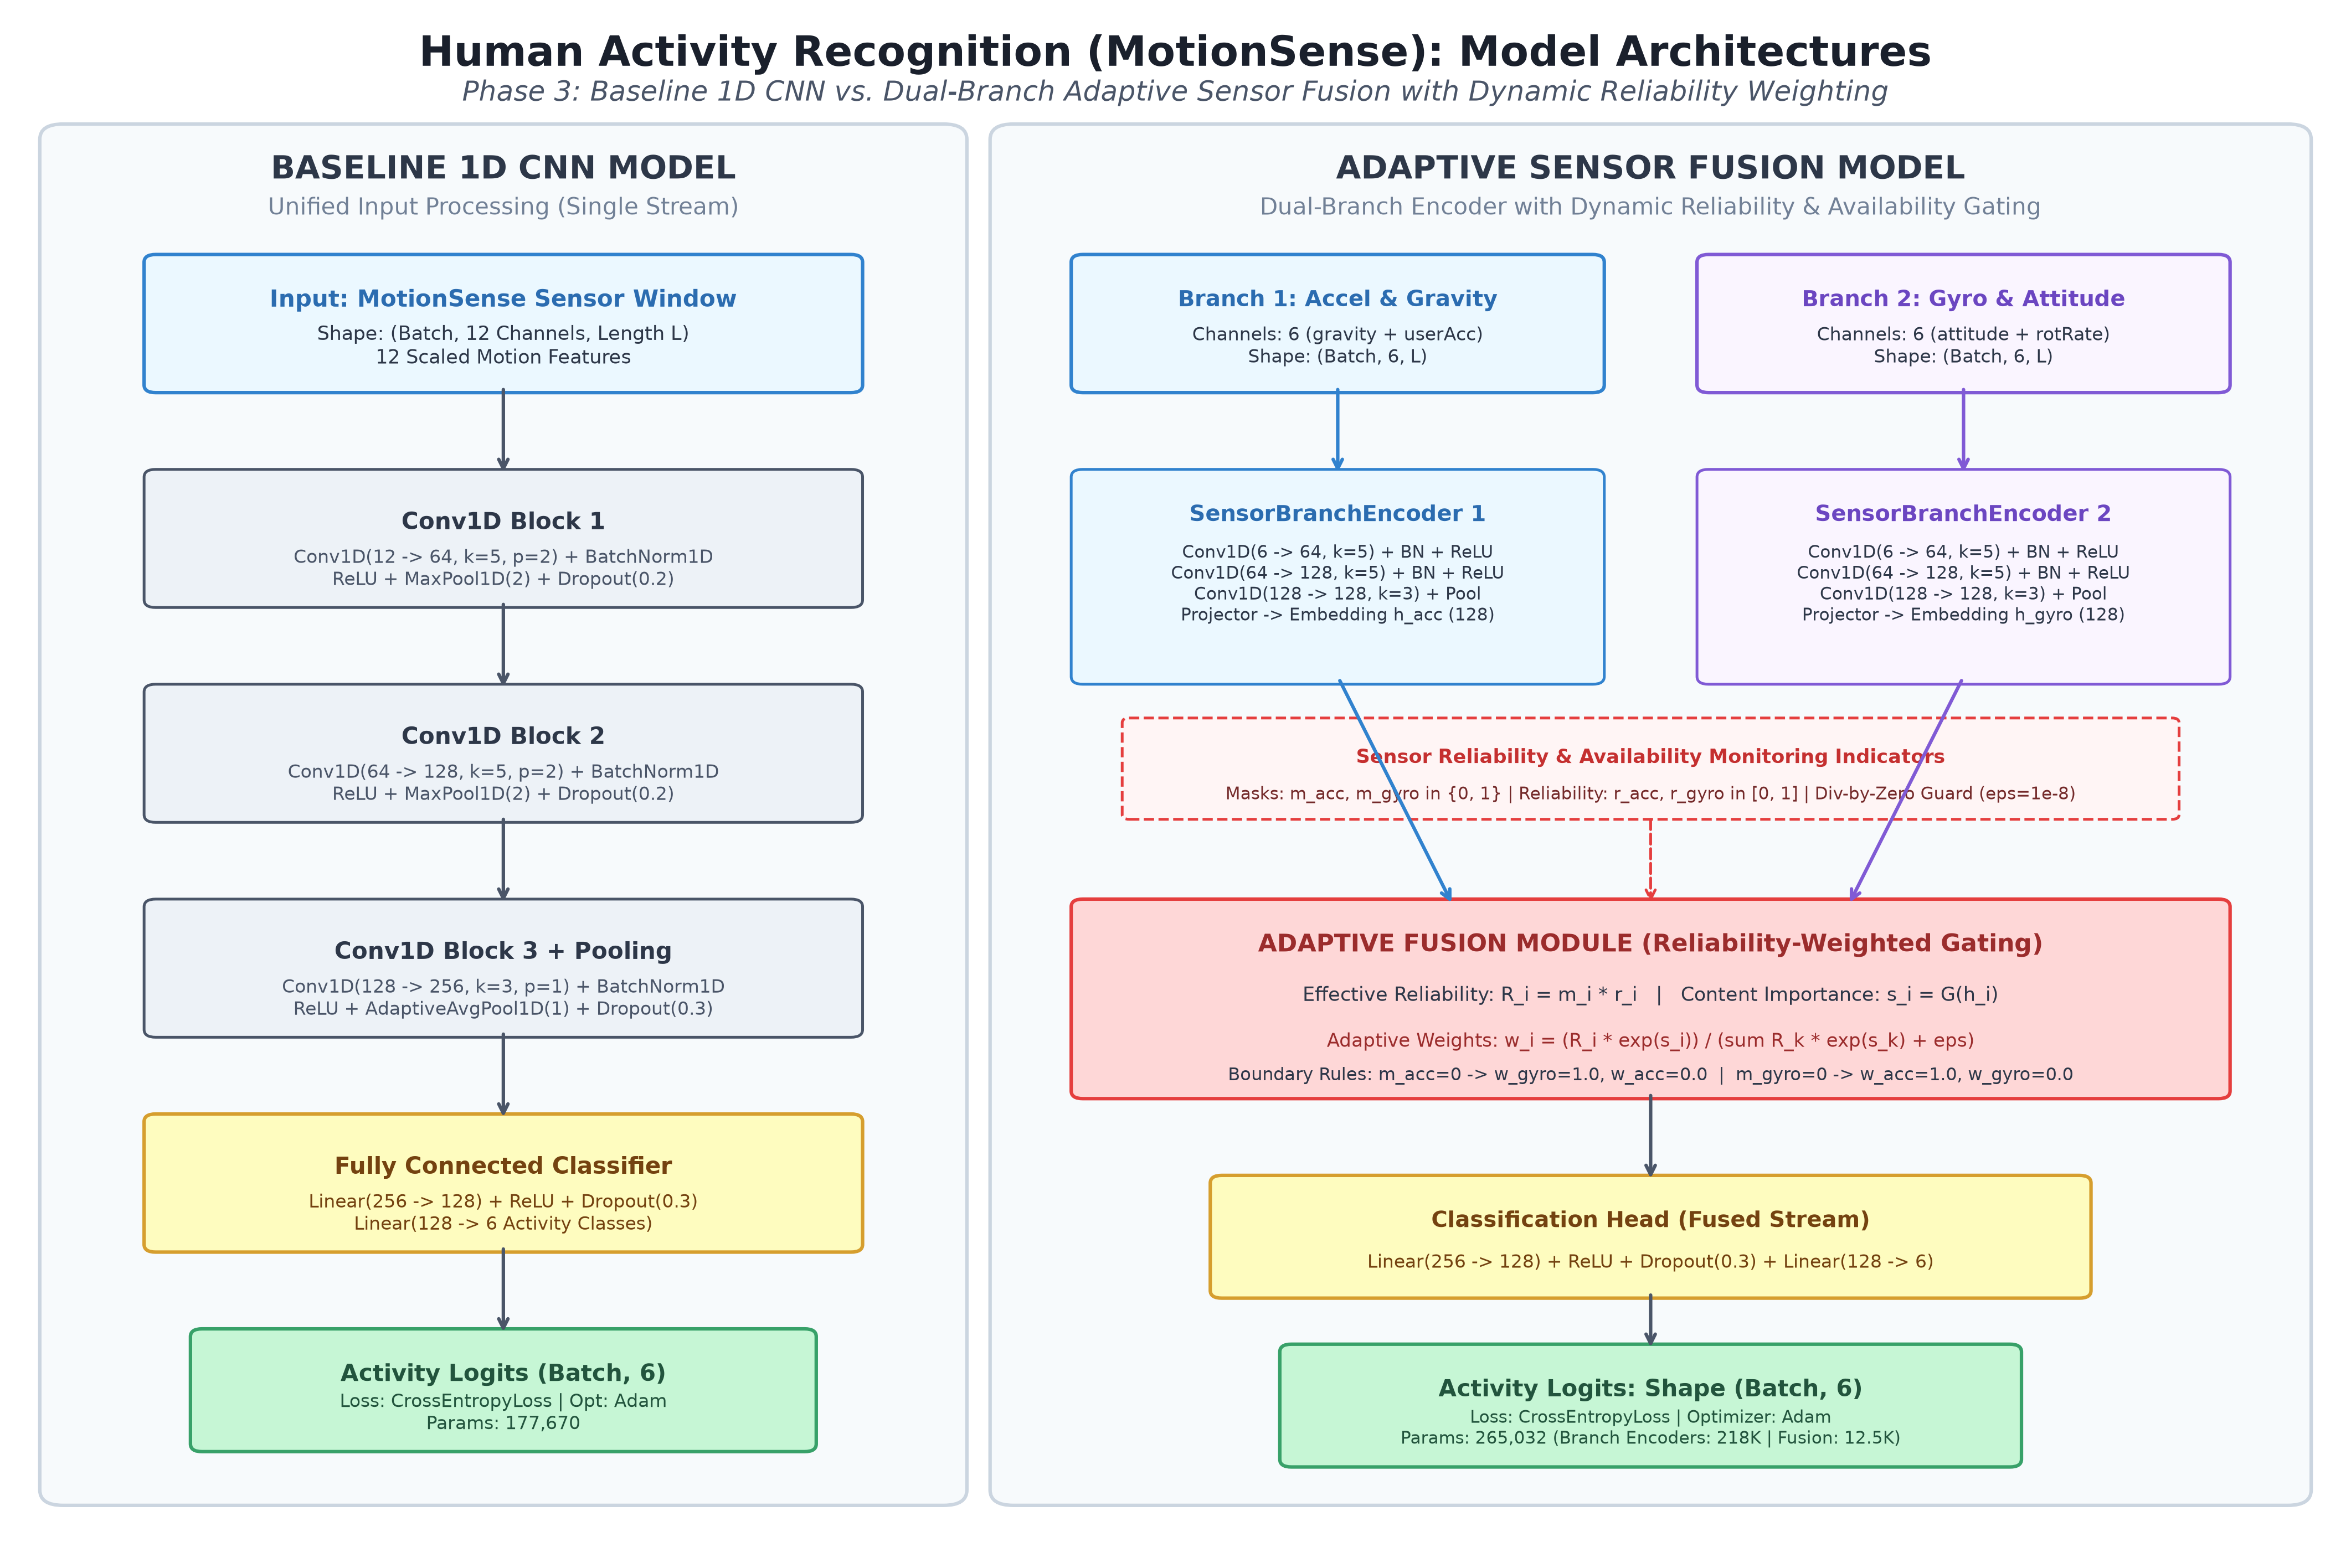
\includegraphics[width=\textwidth]{diagrams/model_architecture.png}
    \caption{Architectural comparison between (Left) the baseline single-stream 1D CNN and (Right) the proposed dual-branch Adaptive Sensor Fusion model with dynamic reliability and availability gating.}
    \label{fig:model_architecture}
\end{figure*}

\subsubsection{Specialized Branch Encoders}
The twelve sensor features are partitioned into two six-dimensional sub-streams:
\begin{align}
    \mathbf{X}_{\text{acc}}  &= \mathbf{X}[:, [3, 4, 5, 9, 10, 11], :] \in \mathbb{R}^{B \times 6 \times L} \\
    \mathbf{X}_{\text{gyro}} &= \mathbf{X}[:, [0, 1, 2, 6, 7, 8], :] \in \mathbb{R}^{B \times 6 \times L}
\end{align}
Each branch employs a dedicated \texttt{SensorBranchEncoder} parameterized by:
\begin{enumerate}
    \item $\text{Conv1D}(6 \to 64, k=5, p=2) \to \text{BatchNorm1d} \to \text{ReLU} \to \text{MaxPool1d}(2) \to \text{Dropout}(0.20)$
    \item $\text{Conv1D}(64 \to 128, k=5, p=2) \to \text{BatchNorm1d} \to \text{ReLU} \to \text{MaxPool1d}(2) \to \text{Dropout}(0.20)$
    \item $\text{Conv1D}(128 \to 128, k=3, p=1) \to \text{BatchNorm1d} \to \text{ReLU} \to \text{AdaptiveAvgPool1d}(1) \to \text{Dropout}(0.20)$
    \item $\text{Linear}(128 \to 128) \to \text{LayerNorm}(128) \to \text{ReLU}$
\end{enumerate}
This yields latent representations $\mathbf{h}_{\text{acc}} \in \mathbb{R}^{B \times 128}$ and $\mathbf{h}_{\text{gyro}} \in \mathbb{R}^{B \times 128}$, each specialized in capturing the physical dynamics of its respective sensor modality.

\subsubsection{Mathematical Formulation of the Adaptive Fusion Mechanism}
Let $m_{\text{acc}}, m_{\text{gyro}} \in \{0, 1\}$ represent binary availability masks indicating whether the physical sensor stream is active ($1$) or disconnected ($0$). Let $r_{\text{acc}}, r_{\text{gyro}} \in [0, 1]$ represent continuous reliability indicators reflecting signal-to-noise ratio, variance stability, or channel confidence. When external reliability metrics are omitted, learned confidence estimators within the network estimate self-confidence directly from branch embeddings:
\begin{equation}
    r_i = \sigma(\mathbf{W}_{\text{conf}, i} \mathbf{h}_i + \mathbf{b}_{\text{conf}, i}), \quad i \in \{\text{acc}, \text{gyro}\}
\end{equation}
where $\sigma(\cdot)$ denotes the logistic sigmoid function.

The effective branch reliability $R_i$ is computed as:
\begin{equation}
    R_{\text{acc}} = m_{\text{acc}} \cdot r_{\text{acc}}, \qquad R_{\text{gyro}} = m_{\text{gyro}} \cdot r_{\text{gyro}}
\end{equation}
Concurrently, content-based relevance scores $s_i$ are extracted via a shared gating projection $G(\mathbf{h}) = \mathbf{W}_g \text{ReLU}(\mathbf{V}_g \mathbf{h} + \mathbf{c}_g) + b_g$:
\begin{equation}
    s_{\text{acc}} = G(\mathbf{h}_{\text{acc}}), \qquad s_{\text{gyro}} = G(\mathbf{h}_{\text{gyro}})
\end{equation}

To avoid numerical overflow, scores are stabilized by subtracting $s_{\max} = \max(s_{\text{acc}}, s_{\text{gyro}})$. Unnormalized dynamic importances are calculated as:
\begin{equation}
    \alpha_{\text{acc}} = R_{\text{acc}} \cdot \exp(s_{\text{acc}} - s_{\max}), \qquad \alpha_{\text{gyro}} = R_{\text{gyro}} \cdot \exp(s_{\text{gyro}} - s_{\max})
\end{equation}
Normalized adaptive fusion weights $w_{\text{acc}}$ and $w_{\text{gyro}}$ are computed using a numerical stabilization guard $\epsilon = 10^{-8}$:
\begin{equation}
    w_{\text{acc}} = \frac{\alpha_{\text{acc}}}{\alpha_{\text{acc}} + \alpha_{\text{gyro}} + \epsilon}, \qquad w_{\text{gyro}} = \frac{\alpha_{\text{gyro}}}{\alpha_{\text{acc}} + \alpha_{\text{gyro}} + \epsilon}
\end{equation}

\subsubsection{Boundary Conditions and Masking Guarantees}
To strictly ensure zero leakage of corrupted data when a sensor modality is unavailable, the mechanism enforces boundary constraints:
\begin{equation}
    (w_{\text{acc}}, w_{\text{gyro}}) = 
    \begin{cases}
        (0.0, 1.0), & \text{if } m_{\text{acc}} = 0 \text{ and } m_{\text{gyro}} = 1 \\
        (1.0, 0.0), & \text{if } m_{\text{gyro}} = 0 \text{ and } m_{\text{acc}} = 1 \\
        (0.5, 0.5), & \text{if } m_{\text{acc}} = 0 \text{ and } m_{\text{gyro}} = 0 \\
        (w_{\text{acc}}, w_{\text{gyro}}), & \text{if } m_{\text{acc}} = 1 \text{ and } m_{\text{gyro}} = 1
    \end{cases}
\end{equation}
The latent embeddings are explicitly modulated:
\begin{equation}
    \mathbf{h}_{\text{acc}}^{\text{eff}} = \mathbf{h}_{\text{acc}} \cdot m_{\text{acc}}, \qquad \mathbf{h}_{\text{gyro}}^{\text{eff}} = \mathbf{h}_{\text{gyro}} \cdot m_{\text{gyro}}
\end{equation}
The fused representation $\mathbf{h}_{\text{fused}} \in \mathbb{R}^{B \times 256}$ concatenates the reliability-modulated features:
\begin{equation}
    \mathbf{h}_{\text{fused}} = \left[ w_{\text{acc}} \cdot \mathbf{h}_{\text{acc}}^{\text{eff}} \;\|\; w_{\text{gyro}} \cdot \mathbf{h}_{\text{gyro}}^{\text{eff}} \right]
\end{equation}
The final classification head maps $\mathbf{h}_{\text{fused}}$ to activity logits:
\begin{equation}
    \hat{\mathbf{y}} = \mathbf{W}_{\text{cls}, 2} \text{Dropout}(\text{ReLU}(\mathbf{W}_{\text{cls}, 1} \mathbf{h}_{\text{fused}} + \mathbf{b}_{\text{cls}, 1}), p=0.3) + \mathbf{b}_{\text{cls}, 2}
\end{equation}
where $\hat{\mathbf{y}} \in \mathbb{R}^{B \times 6}$. The model contains \textbf{265,032} total parameters (Acc Branch: 109,440; Gyro Branch: 109,440; Adaptive Fusion Module: 12,482; Classifier Head: 33,670).

\subsection{Loss Function and Optimization Strategy}
\label{subsec:loss_and_optimizer}

Both architectures are trained using the multiclass \textbf{Cross-Entropy Loss} ($\mathcal{L}_{\text{CE}}$):
\begin{equation}
    \mathcal{L}_{\text{CE}}(\mathbf{y}, \hat{\mathbf{y}}) = -\frac{1}{B} \sum_{i=1}^{B} \sum_{k=1}^{K} y_{i, k} \log \left( \frac{\exp(\hat{y}_{i, k})}{\sum_{j=1}^{K} \exp(\hat{y}_{i, j})} \right)
\end{equation}
where $K = 6$ represents the target activity classes and $\mathbf{y}_i$ is the one-hot encoded ground truth.

For model optimization, we prescribe the \textbf{Adam} (Adaptive Moment Estimation) optimizer configured with an initial learning rate $\eta = 10^{-3}$, decay parameters $\beta_1 = 0.9$, $\beta_2 = 0.999$, numerical stability parameter $\epsilon_{\text{opt}} = 10^{-8}$, and weight decay $L_2$ regularization $\lambda = 10^{-4}$ to prevent overfitting on continuous time-series patterns.

\subsection{How Adaptive Fusion Improves System Reliability}
\label{subsec:reliability_justification}

The adaptive sensor fusion mechanism provides three distinct reliability benefits over conventional single-stream CNNs:
\begin{enumerate}
    \item \textbf{Graceful Degradation under Missing Modalities:} In real-world smartphone usage, sensors may disconnect or experience driver dropouts. In conventional models, zeroing out input channels introduces severe distribution shifts. In \texttt{AdaptiveSensorFusion}, the availability mask triggers boundary enforcement: the disconnected branch weight becomes $0.0$, its latent features are masked out, and the remaining healthy sensor's weight scales to $1.0$, enabling unbroken classification.
    \item \textbf{Noise Immunity via Reliability Gating:} When a sensor produces high-noise measurements (e.g., erratic accelerometer signals during sudden device shocks or loose pocket positioning), the reliability indicator diminishes $r_{\text{acc}}$, shifting fusion weight toward the more stable gyroscope/attitude branch.
    \item \textbf{Preservation of Modality-Specific Representations:} By extracting features through separate, dedicated convolutional filters, spatial orientation semantics (Euler angles and angular velocity) are preserved without destructive interference from high-frequency translational shocks (user acceleration).
\end{enumerate}

